\newcommand{\algorithmicinput}{\textbf{Input}}
\newcommand{\INPUT}{\item[\algorithmicinput]}
\newcommand{\algorithmicoutput}{\textbf{Output}}
\newcommand{\OUTPUT}{\item[\algorithmicoutput]}

\begin{frame}[c]{}

\centering
\huge
Lecture 7:\\
Neural Architecture Search\\
	(Part 1)
\end{frame}
%----------------------------------------------------------------------
\begin{frame}[c]{Where are we? The big picture}

\begin{itemize}
	\item Introduction
	\item Background
	\begin{itemize}
		\item Design spaces in ML
		\item Evaluation and visualization
	\end{itemize}
	\item Hyperparameter optimization (HPO)
	\begin{itemize}
		\item Bayesian optimization
		\item Other black-box techniques
		%\item \strikethrough{Speeding up HPO with multi-fidelity optimization}
		\item More details on Gaussian processes
	\end{itemize}
	\item Pentecost (Holiday) -- no lecture
	\item[$\to$]  Architecture search I + II
	\item Meta-Learning
	\item Learning to learn $\&$ optimize
	\item Beyond AutoML: algorithm configuration and control
	\item Project announcement and closing
\end{itemize}

\end{frame}
%----------------------------------------------------------------------

%----------------------------------------------------------------------
\begin{frame}[c]{Learning Goals}

After this lecture, you will be able to \ldots

\begin{itemize}
	\item describe different \alert{search spaces} for neural architecture search (NAS)
	\item describe various \alert{optimization methods for NAS}
	\item explain various \alert{speedup techniques for NAS}
\end{itemize}


\end{frame}
%-----------------------------------------------------------------------
\section{Motivation and Brief History}
%----------------------------------------------------------------------
\begin{frame}[c]{Motivation for Neural Architecture Search}

\centering
\begin{itemize}
  \item Performance improvements on various tasks mostly due to novel architectural design choices
  \item Designing neural network architectures is hard, requiring lots of human efforts
  \item Can we automate this design process, potentially discovering new components/topologies?
\end{itemize}
	
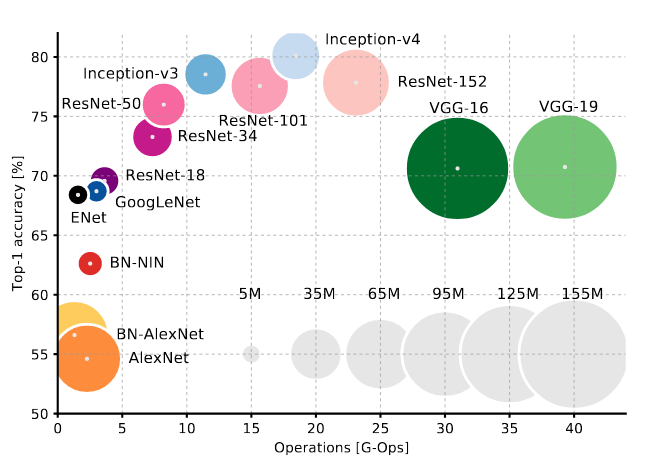
\includegraphics[width=0.5\textwidth]{images_lec7/architectures_perf.png}\\
\lit{Canziani et al. 2017}

\end{frame}
%-----------------------------------------------------------------------
%----------------------------------------------------------------------
\begin{frame}[c]{Successful Human-designed Architectures}

\centering
34-layer ResNet \lit{He et al. 2015}
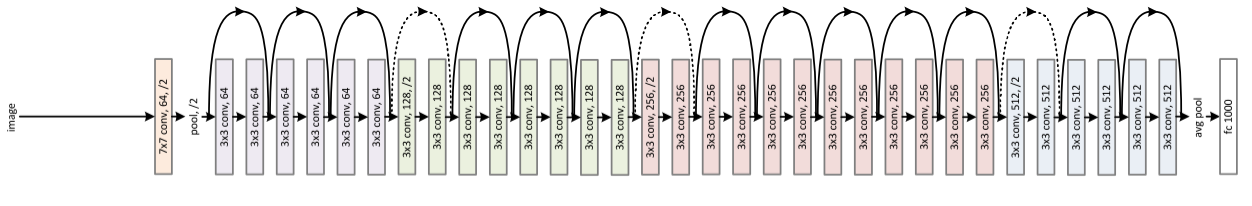
\includegraphics[width=0.8\textwidth]{images_lec7/resnet.png}\\
Inception-v3 \lit{Szegedy et al. 2016}
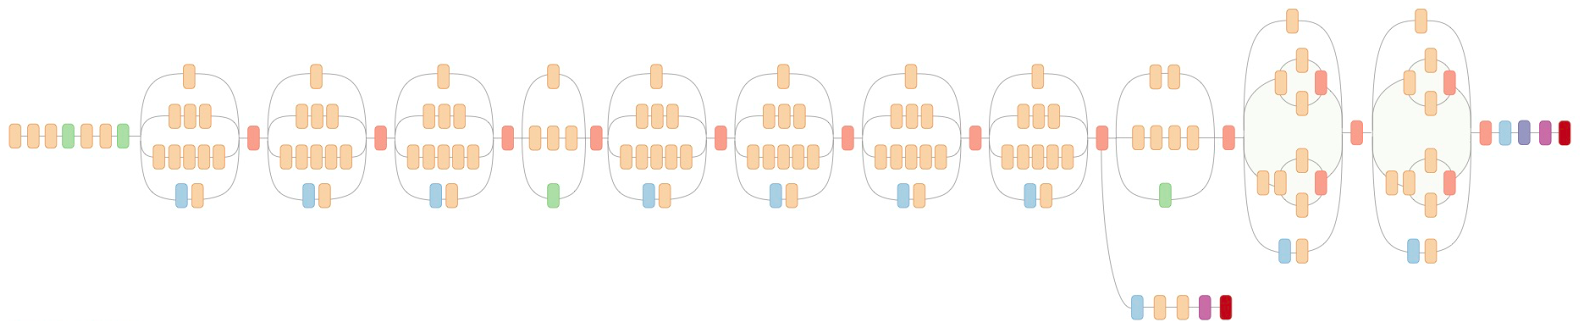
\includegraphics[width=0.8\textwidth]{images_lec7/inception.png}
\pause

\begin{columns}

\column{0.4\textwidth}
ResNet/ResNeXt blocks \lit{He et al. 2015, 2016; Xie et al. 2016}
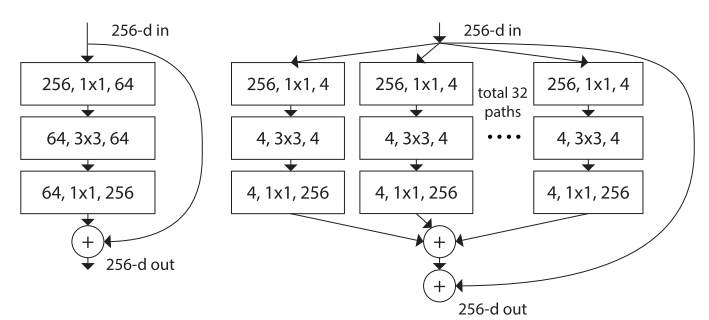
\includegraphics[width=\textwidth]{images_lec7/resnet_block.png}
\column{0.55\textwidth}
Inception-v4 blocks \lit{Szegedy et al. 2017}
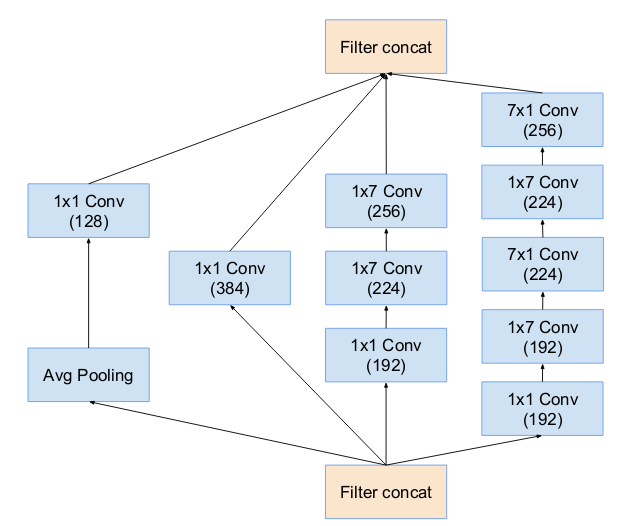
\includegraphics[width=0.4\textwidth]{images_lec7/inception_1.png}
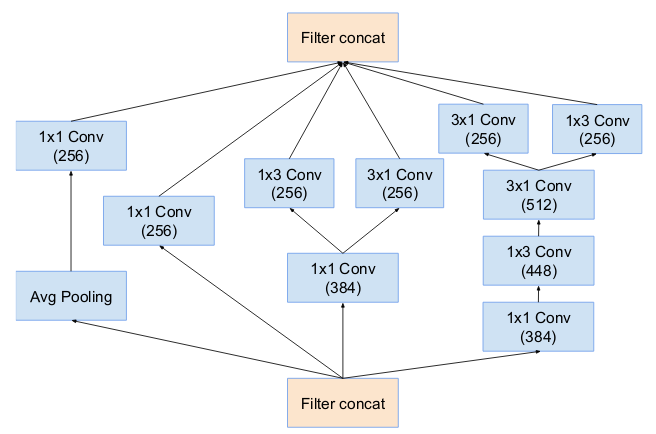
\includegraphics[width=0.4\textwidth]{images_lec7/inception_2.png}

\end{columns}

\end{frame}
%-----------------------------------------------------------------------
%----------------------------------------------------------------------
\begin{frame}[c]{Brief history and early approaches}
\centering
\begin{itemize}
	\item Neuroevolution (already since the 1990s)
	\begin{itemize}
		\item Some authors used evolutionary algorithms for the
		architecture, optimizing the weights with SGD
		\item Others optimized both architecture and weights with
		evolutionary methods
	\end{itemize}
\end{itemize}

%\hspace{1cm}
\begin{columns}
\column{0.47\textwidth}
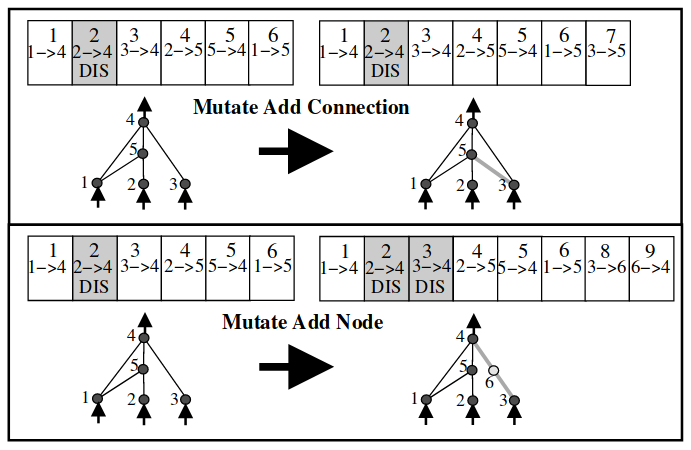
\includegraphics[width=0.9\textwidth]{images_lec7/neat.png}
\column{0.4\textwidth}
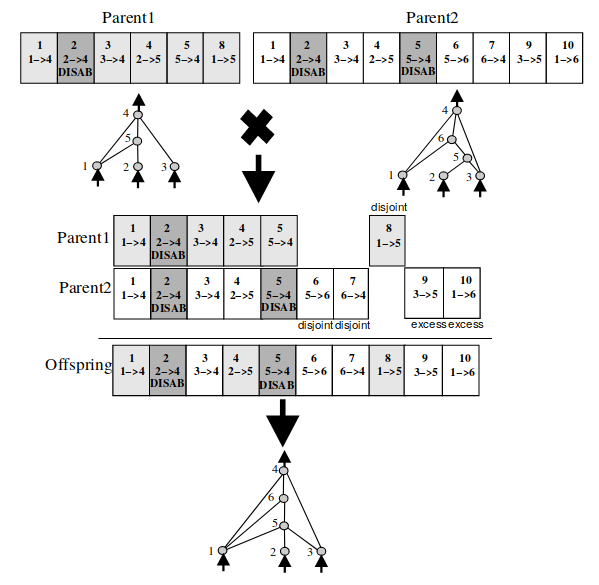
\includegraphics[width=0.8\textwidth]{images_lec7/neat_2.png}
\end{columns}
\end{frame}
%-----------------------------------------------------------------------
%----------------------------------------------------------------------
\begin{frame}[c]{Brief history and early approaches}
\begin{itemize}
	\item Bayesian optimization
	\begin{itemize}
		\item Bergstra et al, 2013: optimized 238 hyperparameters of a vision
		architecture with TPE
		\item Domhan et al. 2015: optimized CNN with up to 6 layers with SMAC
		\begin{itemize}
			\item[--] \alert{81 hyperparameters} including 9 network 
			and 12 architectural layer-wise hyperparameters. 
			\item[--] New best results on CIFAR-10 without data augmentation
		\end{itemize}
		\item Mendoza et al, 2016: joint optimization of architecture and
		hyperparameters in fully-connected network
		\begin{itemize}
			\item[--] \alert{29 hyperparameters} including 14 network and 15 
			architectural layer-wise hyperparameters.
			\item[--] First Auto-DL system to win a competition dataset against 
			human experts.
		\end{itemize}
	\end{itemize}
\end{itemize}
\end{frame}
%-----------------------------------------------------------------------
%----------------------------------------------------------------------
\begin{frame}[c]{Since Then: Many Works on Architecture Search}
\centering
	\begin{itemize}
		\item RL \& Evolution for NAS by Google Brain \lit{Quoc Le’s group, ‘16-’18}
		\begin{itemize}
			\begin{footnotesize}
			\item New state-of-the-art results for
			CIFAR-10, ImageNet, Penn Treebank
			\item Large computational demands
			\begin{itemize}
				\item[--] \alert{800 GPUs for 2 weeks; 12800 architectures evaluated}
			\end{itemize}
			\item Hyperparameter optimization only as postprocessing
			\end{footnotesize}
		\end{itemize}
		\pause

		\item NAS for dense prediction, video classification and machine translation
		\begin{itemize}
			\begin{footnotesize}
			\item AutoDeepLab for semantic segmentation and AutoDispNet for
			disparity estimation tasks \lit{Liu et al.’18; Saikia et al.’19}
			\item Improved accuracy for action classification on Charades and 
			Moments in Time datasets with AssembleNet \lit{Ryoo et al.’19}
			\item SOTA results in translation tasks with Evolved Transformer 
			\lit{So et al.’19}
			\end{footnotesize}
		\end{itemize}
		\pause

		\item \alert{Recent work aims for efficiency}
		\begin{itemize}
			\begin{footnotesize}
			\item Weight sharing \lit{Pham et al,’18; Bender et al, ’18; Liu et al, ‘19; Xie et al. ’19; Cai et al. ’19, Zhang et al. ’19}
			\item Network morphisms \lit{Chen et al, ’16; Cai et al, ’17 \& ‘18; Elsken et al, ’17 \& 18}
			\item Multi-fidelity optimization \lit{Klein et al, ‘16; Li et al, ‘18; Falkner et al, ‘18}
			\end{footnotesize}
		\end{itemize}
	\end{itemize}
\end{frame}
%----------------------------------------------------------------------
%----------------------------------------------------------------------
%-----------------------------------------------------------------------
\section{Search Space Design}
%-----------------------------------------------------------------------
\begin{frame}[c]{NAS components}

\centering
%\hspace{1cm}
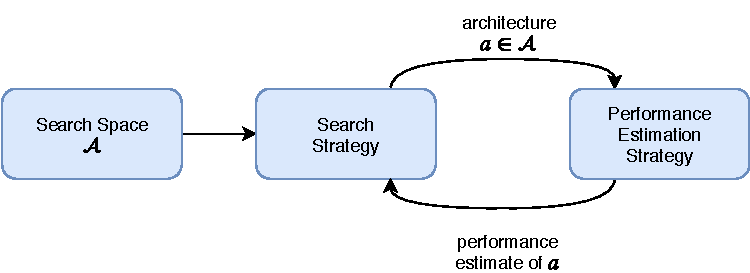
\includegraphics[width=0.9\textwidth]{images_lec7/NAS_diagram.pdf}

\begin{itemize}
	\item \alert{Search Space:} \textit{macro} or \textit{micro} search space
	\item \alert{Search Strategy:} blackbox (RL, ES, BO, etc.) or gradiend-based methods
	\item \alert{Performance Estimation Strategy:} Lower fidelity estimates, curve extrapolation, etc.
\end{itemize}

\end{frame}
%----------------------------------------------------------------------
%-----------------------------------------------------------------------
\begin{frame}[c]{Basic Neural Architecture Search Spaces}
\centering
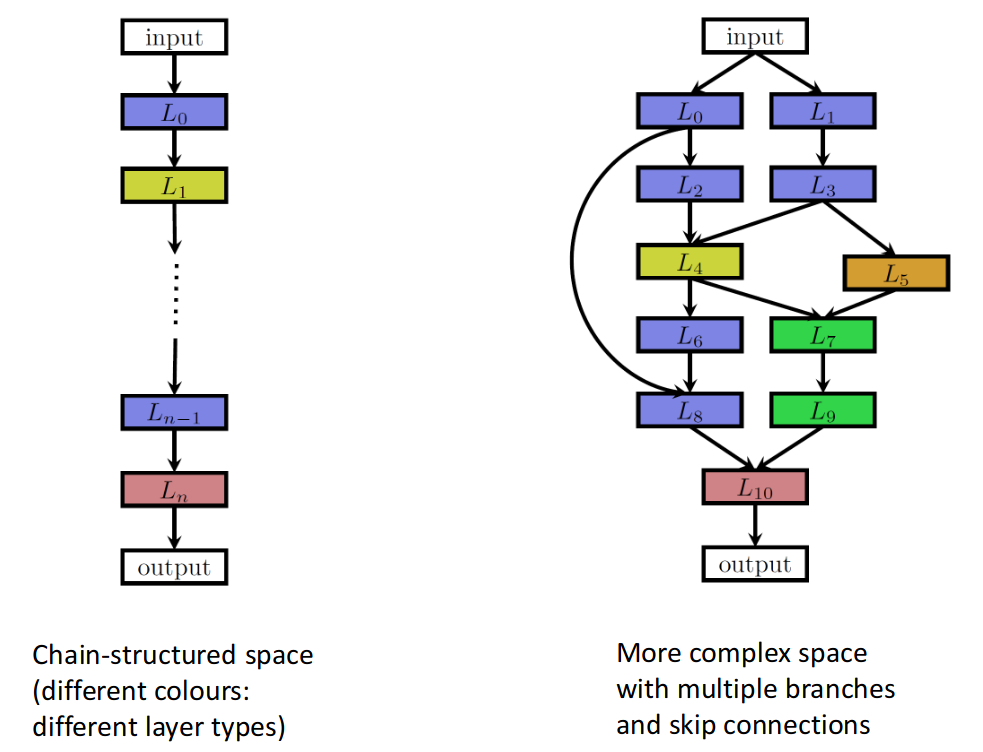
\includegraphics[height=0.9\textheight]{images_lec7/macro_space.png}
\end{frame}
%----------------------------------------------------------------------
%----------------------------------------------------------------------
\begin{frame}[c]{Cell Search Spaces}
\centering
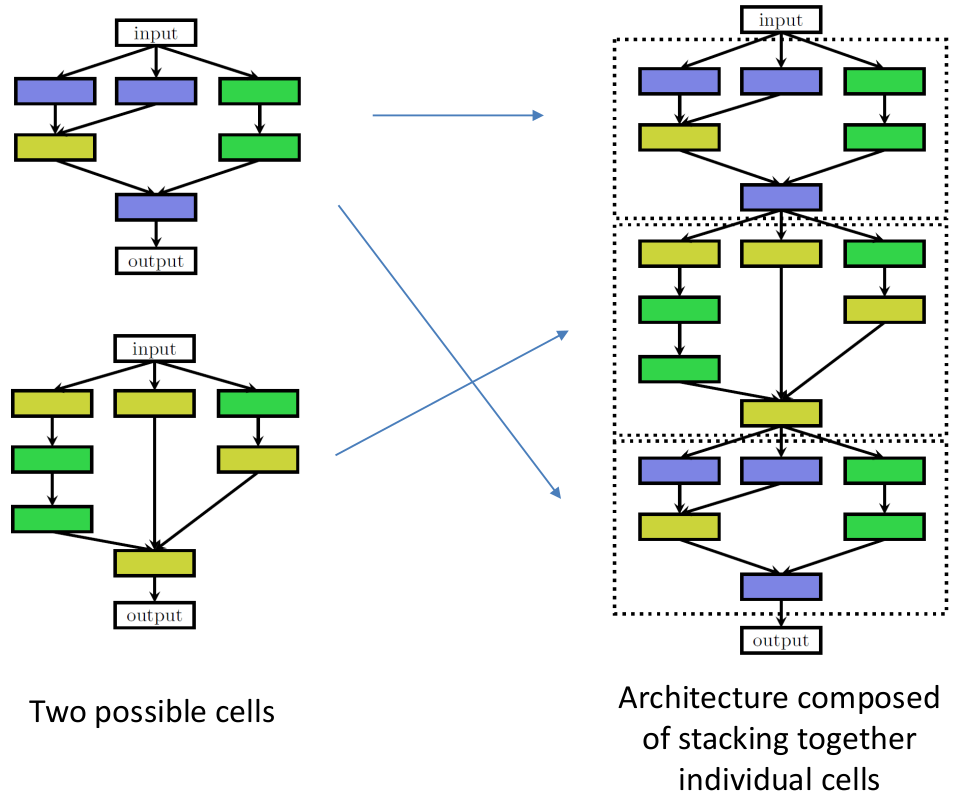
\includegraphics[height=.8\textheight]{images_lec7/s26}\\
Introduced by Zoph et al.’18
\end{frame}
%----------------------------------------------------------------------
%----------------------------------------------------------------------
\begin{frame}[c]{Pros and Cons of Cell Search Space}
\centering
What are some pros and cons of the cell search space compared to the chain-structured one? [2min]\\
%\bigskip
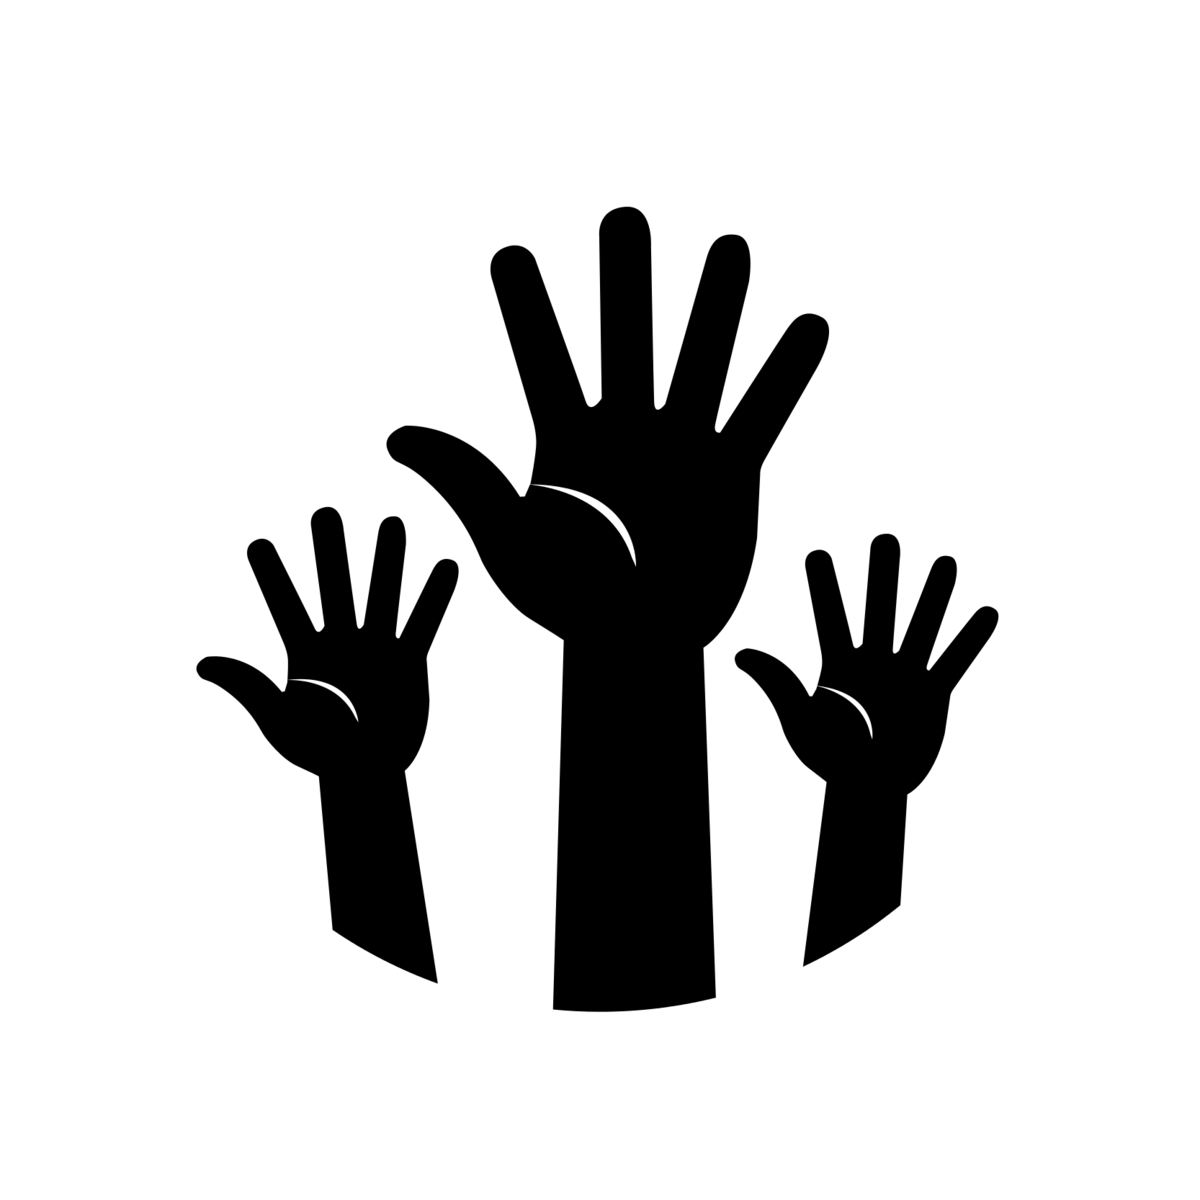
\includegraphics[height=.3\textheight]{images/hands.png}\\
\end{frame}
%----------------------------------------------------------------------
%----------------------------------------------------------------------
\begin{frame}[c]{Pros and Cons of Cell Search Space}
\centering
\alert{Pros:}
\begin{itemize}
	\item[--] Reduced search space size; speed-ups in term of search time.
	\item[--] Transferrability to other datasets (e.g. cells found on
	CIFAR-10 transferred to ImageNet)
	\item[--] Stacking repeating patterns proven to be useful design principle 
	(ResNet, Inception, etc.)
\end{itemize}
\pause
\alert{Cons:}
\begin{itemize}
	\item[--] Manually determining the \textit{macro} architecture, 
	i.e. the way cells are connected.
\end{itemize}

\end{frame}
%----------------------------------------------------------------------
%----------------------------------------------------------------------
\begin{frame}[c]{Hierarchical representation of search space \litw{Liu et al.’17}}
\centering
\begin{itemize}
	\item[--] Directed Acyclic Graph (DAG) representation of architectures
	\item[--] Each node a latent representation; each edge an operation/motif
	\item[--] Multiple levels of hierarchy for motifs; e.g. $o_1^{(2)}$ is a level-2 motif, 
	$o_1^{(3)}$ is a level-3 motif
\end{itemize}
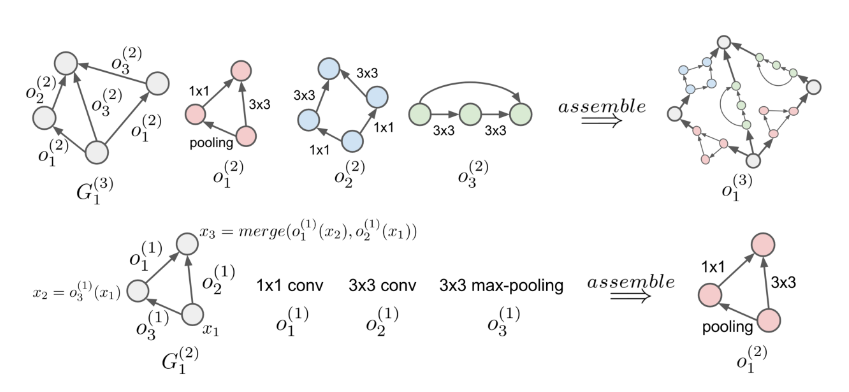
\includegraphics[width=\textwidth]{images_lec7/hierarchical_nas.png}\\
\end{frame}
%----------------------------------------------------------------------
%----------------------------------------------------------------------

%-----------------------------------------------------------------------
\section{Blackbox Optimization for Neural Architecture Search}
%-----------------------------------------------------------------------
\begin{frame}[c]{Reinforcement Learning \litw{Zoph \& Le, ICLR 2017}}
\centering
\begin{itemize}
	\item Key idea: Use a configuration string to represent the structure and connections in a NN
	\begin{itemize}
		\item[--] E.g.: ["Input to layer 1: 0", "Input to layer 2: 0", "Layer 2: conv"]
	\end{itemize}
	\item Use RNN ("\alert{Controller}") to generate this string that specifies the NN
	\item Train this NN ("\alert{Child Network}") and see how it performs on validation set
	\item Use \alert{REINFORCE/PPO} to update the parameters of the Controller RNN based on the performance of
	child models
\end{itemize}

{\centering
	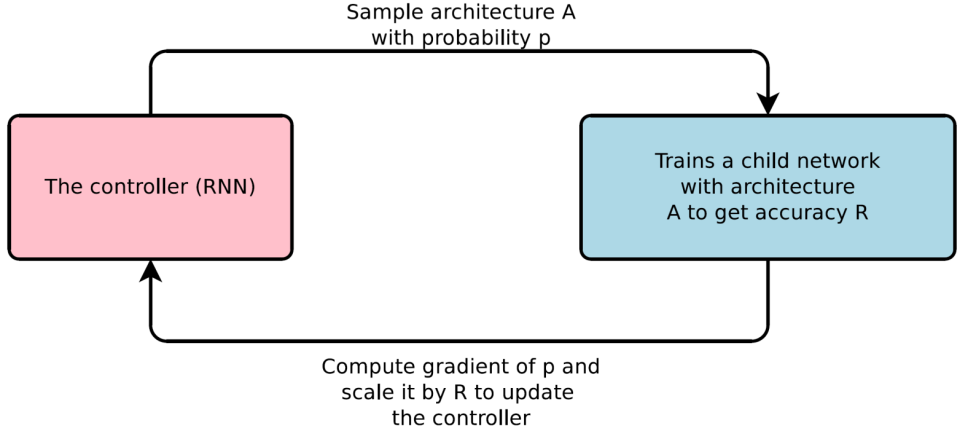
\includegraphics[width=.6\textwidth]{images_lec7/s27}
}
\end{frame}
%----------------------------------------------------------------------
%----------------------------------------------------------------------
\begin{frame}[c]{Learning CNNs with RL \litw{Zoph \& Le, ’17}}
\centering
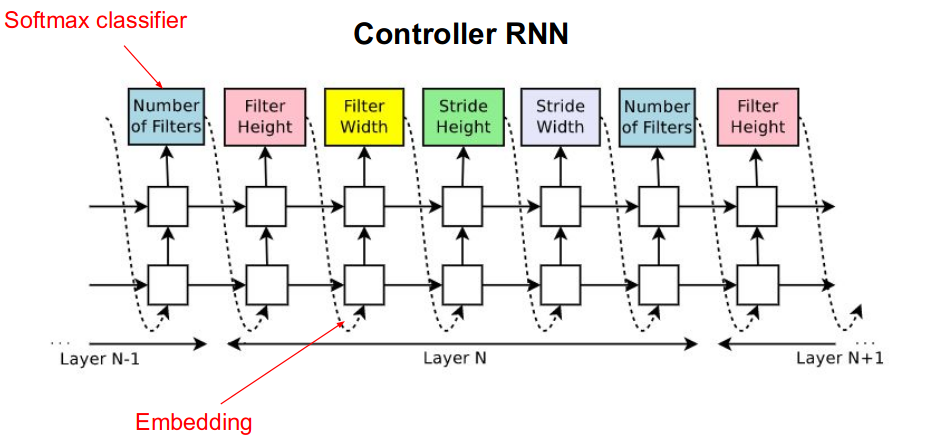
\includegraphics[width=.8\textwidth]{images_lec7/RL_CNN_controller}

\begin{itemize}
\footnotesize{
	\item Maximize expected reward (validation accuracy): 
	$J(\theta_c)=E_{P(a_{1:T; \theta_c})}[R]$
	\item For a fixed number of layers predict:
	\begin{itemize}
		\item[--] Filter width/height, stride width/height, number of filters	
	\end{itemize}
	\item Each child model was trained for 50 epochs
	
}
\end{itemize}
\end{frame}
%----------------------------------------------------------------------
%----------------------------------------------------------------------
\begin{frame}[c]{Learning CNNs with RL \litw{Zoph \& Le, ’17}}
\centering
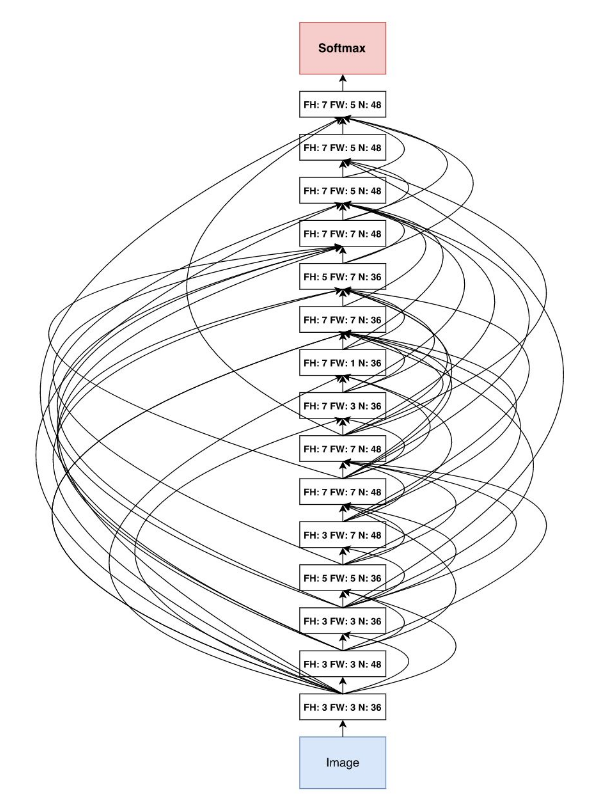
\includegraphics[width=.3\textwidth]{images_lec7/RL_CNN}
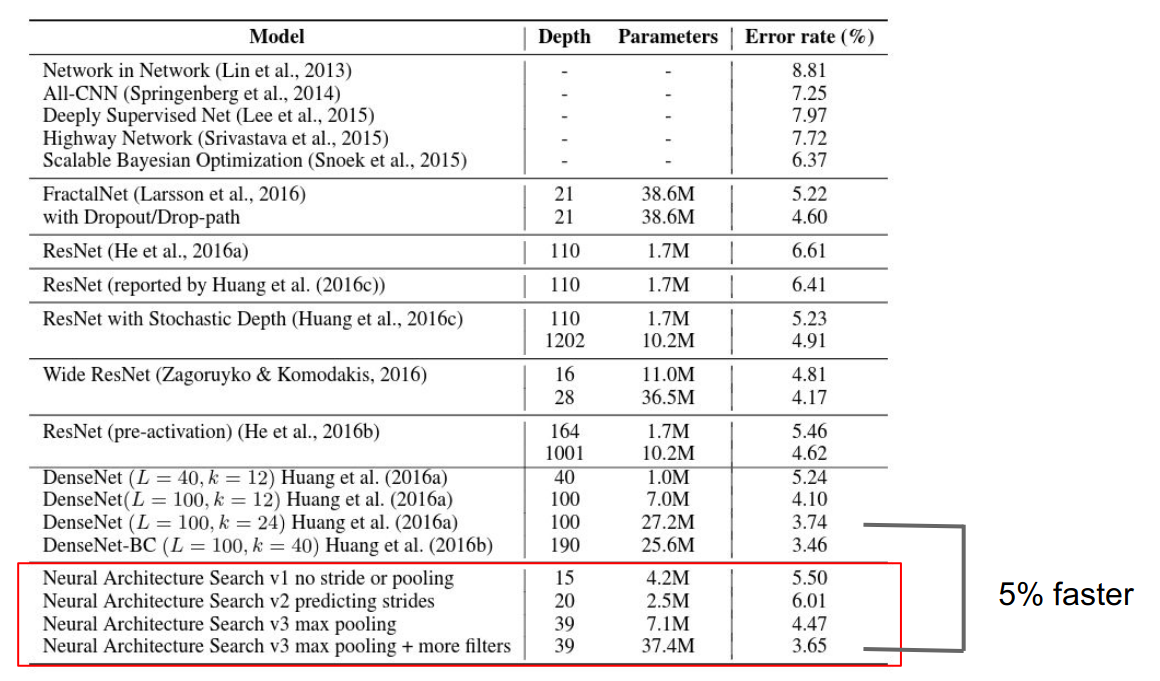
\includegraphics[width=.69\textwidth]{images_lec7/RL_results_table}

\begin{itemize}
\footnotesize{
	\item State-of-the-art results for CIFAR-10, Penn Treebank
	architecture, optimizing the weights with SGD
	\item Large computational demands \alert{800 GPUs for 2 weeks, 
	12.800 architectures evaluated}
	\item Hyperparameter optimization only as postprocessing
}
\end{itemize}
\end{frame}
%----------------------------------------------------------------------
%----------------------------------------------------------------------

\begin{frame}[c]{Learning CNN cells with RL \litw{Zoph et al. ’18}}
\centering

\begin{itemize}
	\footnotesize{
	\item RNN controller makes $2\times 5B$ softmax predictions in total 
	(5B for \textit{normal} and 5B for \textit{reduction} cells)
	\item Determines both topology and operations in each node of the graph
	}
\end{itemize}
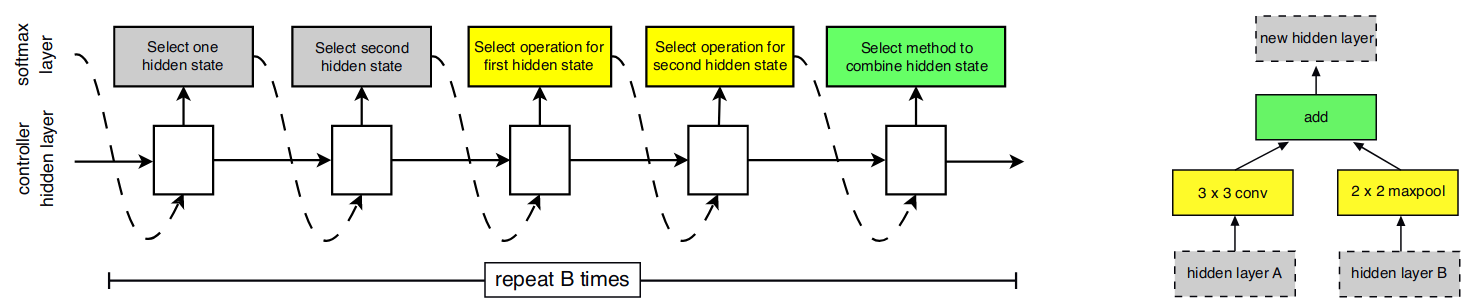
\includegraphics[width=.8\textwidth]{images_lec7/RL_conv_cell}
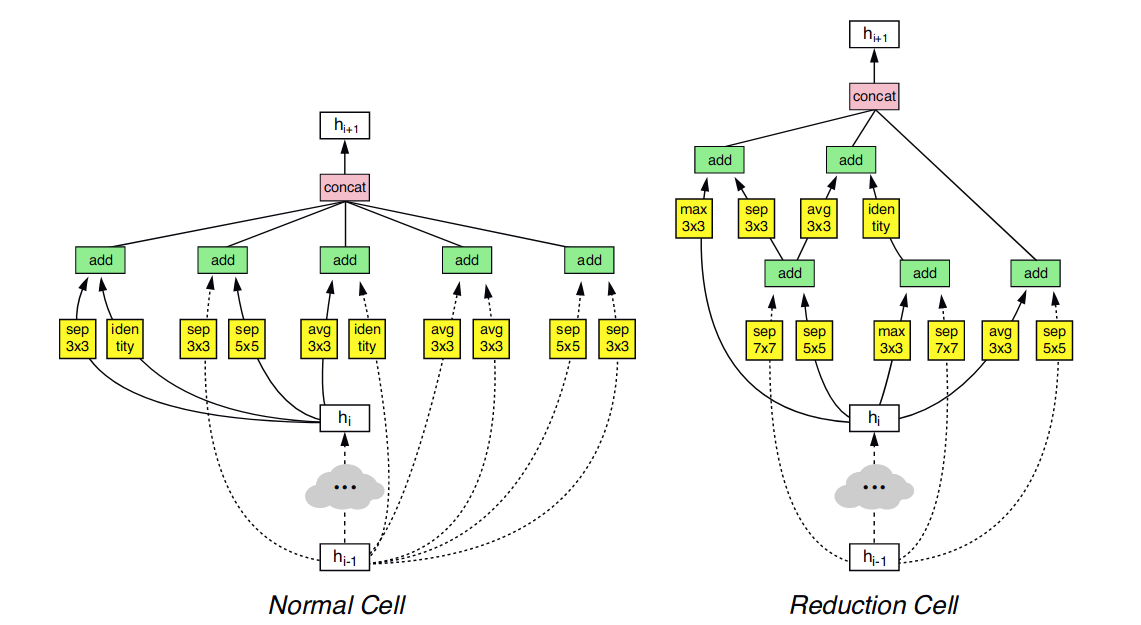
\includegraphics[width=.7\textwidth]{images_lec7/RL_normal_reduction}

\end{frame}
%----------------------------------------------------------------------
%----------------------------------------------------------------------

\begin{frame}[c]{NAS as Hyperparameter Optimization}
\begin{itemize}
	\item Chain-structured space:
	\begin{itemize}
		\item Hyperparameters of layer $k$ conditional on depth $\geq k$
	\end{itemize}
	\item Cell search space
	\begin{itemize}
		\item Fixed (or maximum) number of layers per cell (e.g., 5)
		\item For each: categorical choice between various operations, e.g.,
		between \{conv3x3, conv5x5, max pool, separable conv3x3, ...\}
	\end{itemize}
\end{itemize}

\end{frame}

%----------------------------------------------------------------------
%----------------------------------------------------------------------

\begin{frame}[c]{Evolution}
\centering
\begin{itemize}
\item \alert{Neuroevolution} (already since the 1990s)
\begin{itemize}
	\item[--] Typically optimized both architecture and weights with evolutionary methods
	\lit{Angeline et al. 1994; Stanley and Miikkulainen, 2002}
	\item[--] Mutation steps, such as adding, changing or removing a layer
	\lit{Real et al. ’17; Liu et al. ’17; Miikkulainen et al. ’17}
\end{itemize}
\end{itemize}
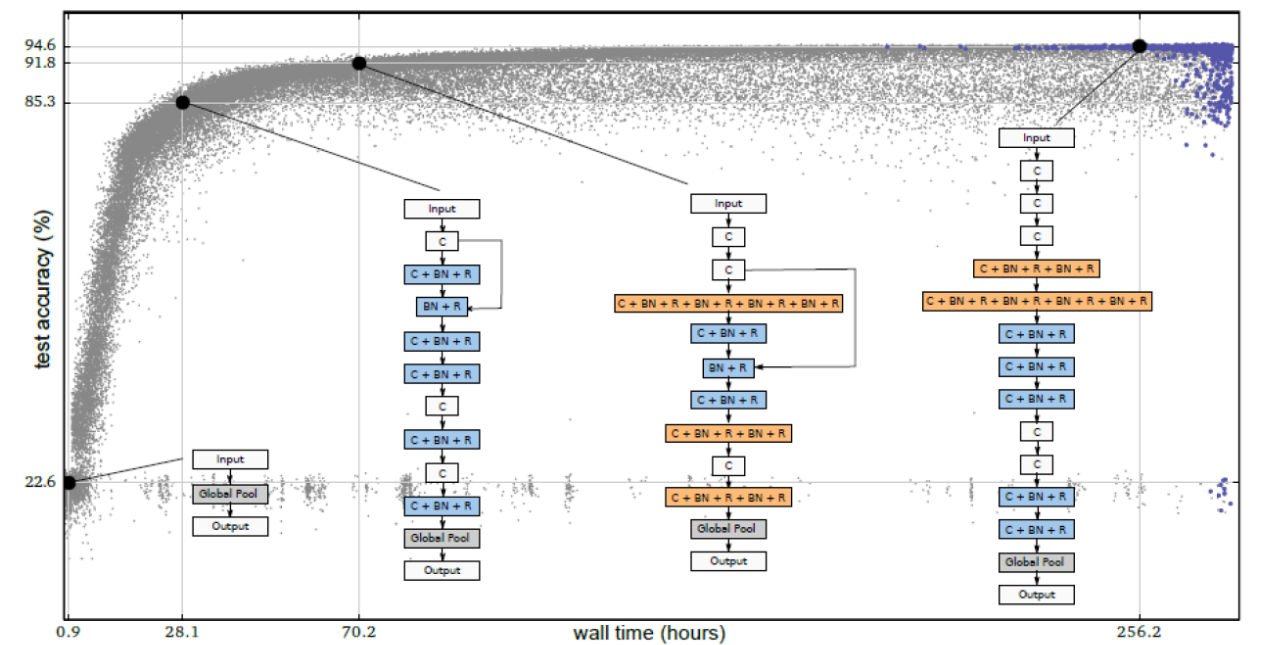
\includegraphics[width=.8\textwidth]{images_lec7/neuroevolution.png}\\
\end{frame}
%----------------------------------------------------------------------
%----------------------------------------------------------------------
\begin{frame}[c]{Regularized/Aging Evolution \litw{Real et al. ’19}}

\centering
\begin{itemize}
	\item Standard evolutionary algorithm, but oldest solutions are dropped from
	population P, instead of the worst.
	\item Same cell search space as in Zoph et al ’18\\
\end{itemize}

\begin{columns}[T]

\column{0.4\textwidth}
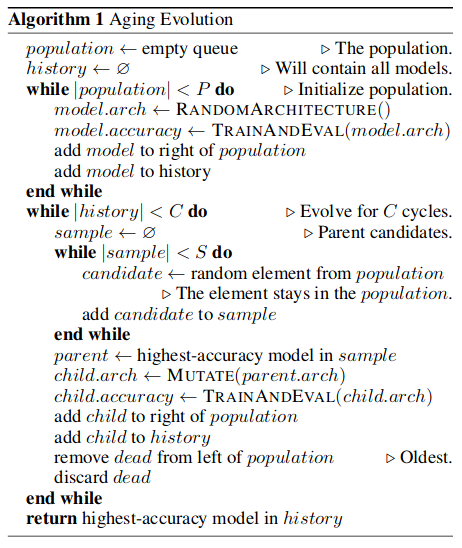
\includegraphics[width=\textwidth]{images_lec7/aging_evolution_alg.png}

\column{0.4\textwidth}
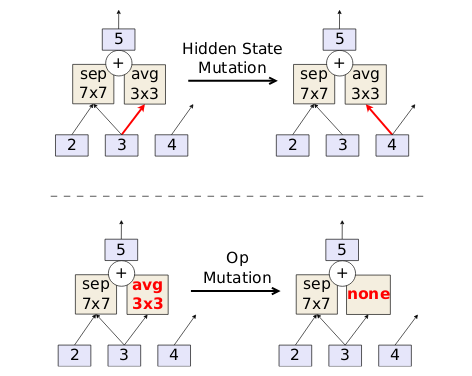
\includegraphics[width=1.1\textwidth]{images_lec7/aging_evolution_mutations.png}

\end{columns}

\end{frame}
%----------------------------------------------------------------------
%----------------------------------------------------------------------
\begin{frame}[c]{Regularized/Aging Evolution \litw{Real et al. ’19}}

\centering
\begin{columns}[T]

\column{0.45\textwidth}
\begin{itemize}
	\footnotesize{
	\item Better results compared to the RL and RS baselines on CIFAR-10 (AmoebaNet-A).
	\item State-of-the-art results on CIFAR-10 when ran on larger search space (AmoebaNet-B/C)
	}
\end{itemize}

\column{0.4\textwidth}
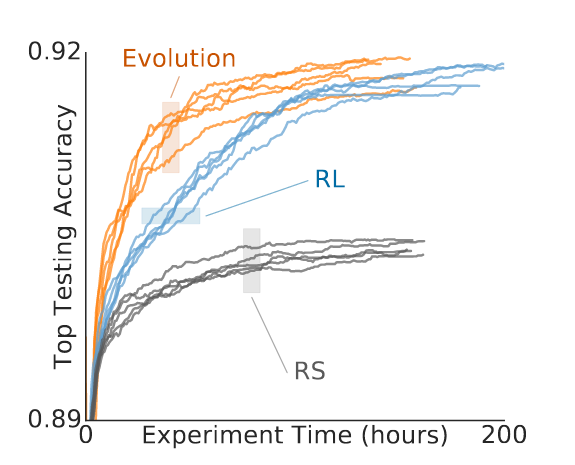
\includegraphics[width=.9\textwidth]{images_lec7/aging_evolution_results.png}

\end{columns}
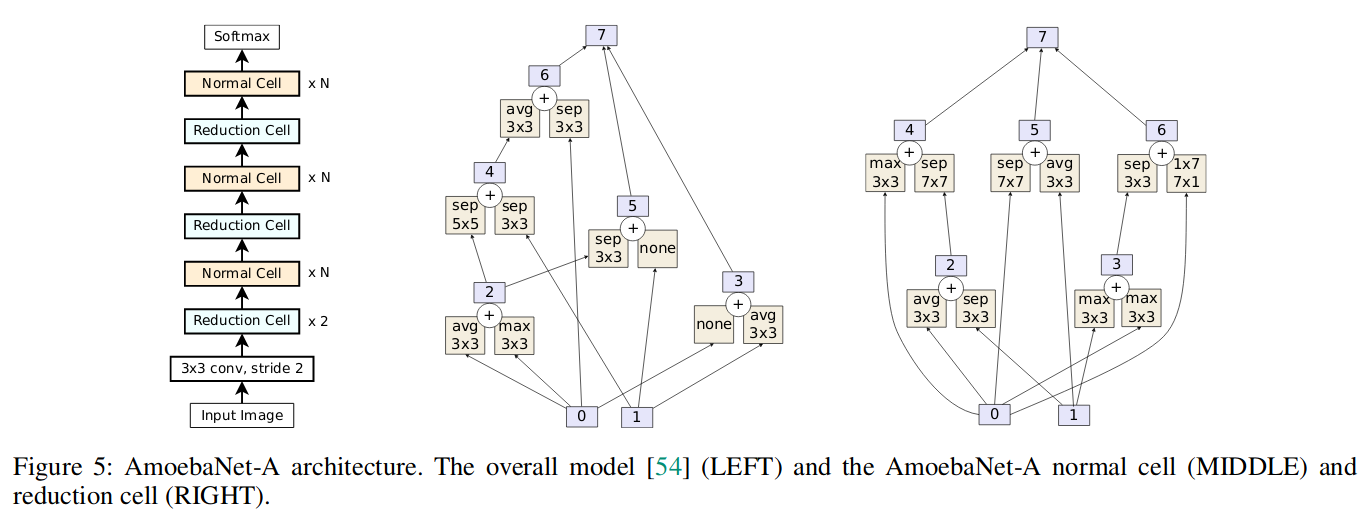
\includegraphics[width=.9\textwidth]{images_lec7/amoebanet_A.png}

\end{frame}
%----------------------------------------------------------------------
%----------------------------------------------------------------------
\begin{frame}[c]{Bayesian Optimization}
\begin{itemize}
	\item \alert{Joint optimization of a vision architecture} with 238 hyperparameters 
	using TPE \lit{Bergstra et al. ’13}
	\item \alert{Auto-Net}
	\begin{itemize}
		\item Joint architecture and hyperparameter search with SMAC
		\item First Auto-DL system to win a competition dataset 
		against human experts \lit{Mendoza et al. ’16}
	\end{itemize}
	\item \alert{Kernels for GP-based NAS}
	\begin{itemize}
		\item Arc kernel \lit{Swersky et al. ’13}
		\item NASBOT \lit{Kandasamy et al. ’18}
	\end{itemize}
	\item \alert{Sequential model-based optimization}
	\begin{itemize}
		\item PNAS \lit{Liu et al. ’18}
	\end{itemize}
\end{itemize}

\end{frame}

%----------------------------------------------------------------------
%----------------------------------------------------------------------

%-----------------------------------------------------------------------
\section{Beyond Blackbox Optimization}
%-----------------------------------------------------------------------
\begin{frame}[c]{Efficient NAS by performance estimation speedup}
\centering
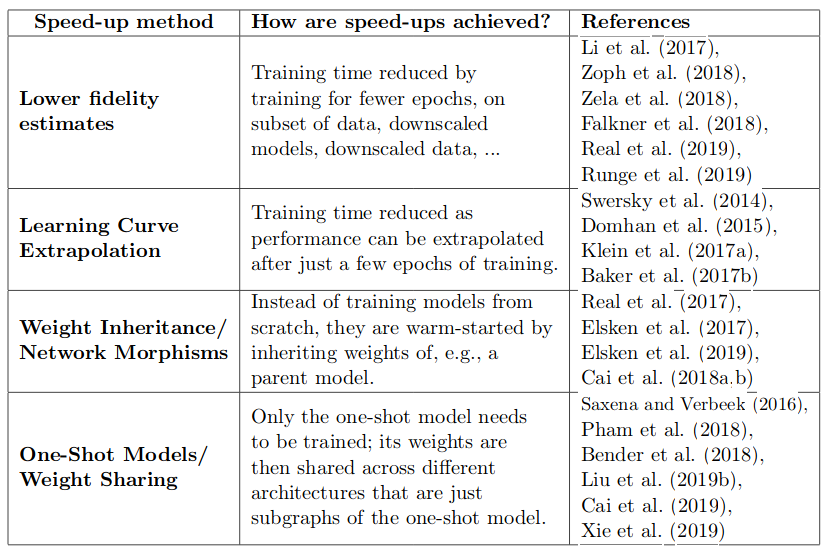
\includegraphics[width=0.9\textwidth]{images_lec7/performance_estimation.png}\\
\end{frame}
%----------------------------------------------------------------------
%----------------------------------------------------------------------
%\begin{frame}[c]{One-shot NAS}
%\centering
%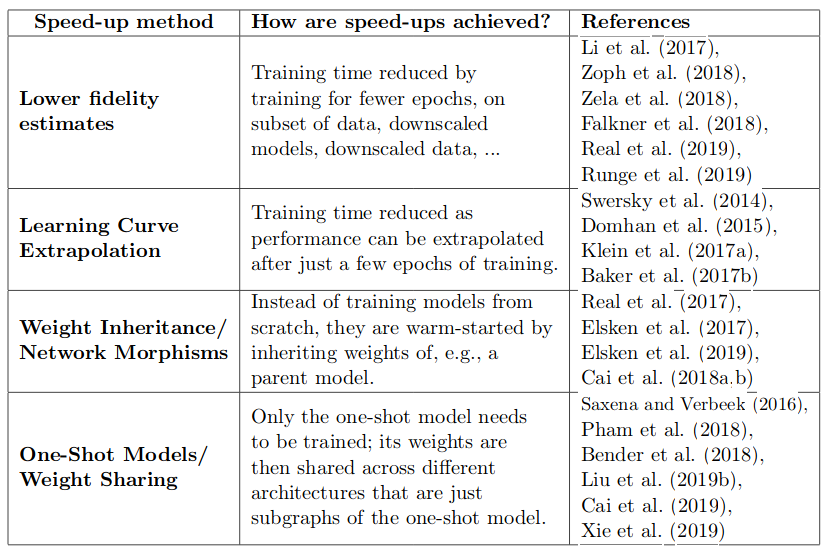
\includegraphics[width=0.9\textwidth]{images_lec7/performance_estimation.png}\\
%\end{frame}
%----------------------------------------------------------------------
%----------------------------------------------------------------------
\begin{frame}[c]{Weight Sharing and One-shot Models}
\centering
	\begin{itemize}
	\item All possible architectures are subgraphs of a large supergraph 
	(the \alert{one-shot model})
	\item \alert{Weights are shared} between different architectures with common edges/nodes in the supergraph
	\item \alert{Search costs reduced} drastically since one only has to train one model (the one-shot model).\\
	\only<1>{\centering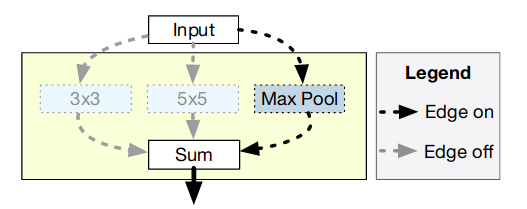
\includegraphics[width=0.5\textwidth]{images_lec7/one_shot_nas.png}}
	\pause
	\item Different one-shot NAS methods differ in how the train the one-shot model and sample
	from it:
	\begin{itemize}
            \item[$\Rightarrow$] ENAS \lit{Pham et al. ’18} uses an RL controller to sample architectures from the supergraph and trains the one-shot model using on approximate gradients obtained through REINFORCE
            \item[$\Rightarrow$] Bender et al. (’18) only train the one-shot model and sample architectures in the end
	    \item[$\Rightarrow$] DARTS (Differentiable Architecture Search; \lit{Liu et al. ’18}) creates a continuous relaxation of the discrete architecture space and optimizes the architecture distribution with gradient descent
	\end{itemize}
	\end{itemize}
	
\end{frame}

%----------------------------------------------------
\begin{frame}[c]{DARTS: Cell Search Space}

	\begin{itemize}
	\only<1>{
	\item 2 cell types
	\begin{itemize}
            \item[$\Rightarrow$] \alert{Normal} - keep spatial resolution unchanged.
            \item[$\Rightarrow$] \alert{Reduction} - reduce spatial resolution by a factor of 2.
        \end{itemize}
        \item Cell $C_k$ gets as input the output of cells $C_{k-1}$ and $C_{k-2}$}
        \only<2>{
	\item DAG (Multigraph) representation
	\begin{itemize}
            \item[$\Rightarrow$] \alert{Nodes} - lattent representations.
            \item[$\Rightarrow$] \alert{Edges (dashed)} - operations.
        \end{itemize}
        \item Architecture optimization problem: \alert{Find optimal path from the input to the output cell}}
	\end{itemize}
	
	\begin{figure}[t]
	\begin{centering}
		\only<2>{
    	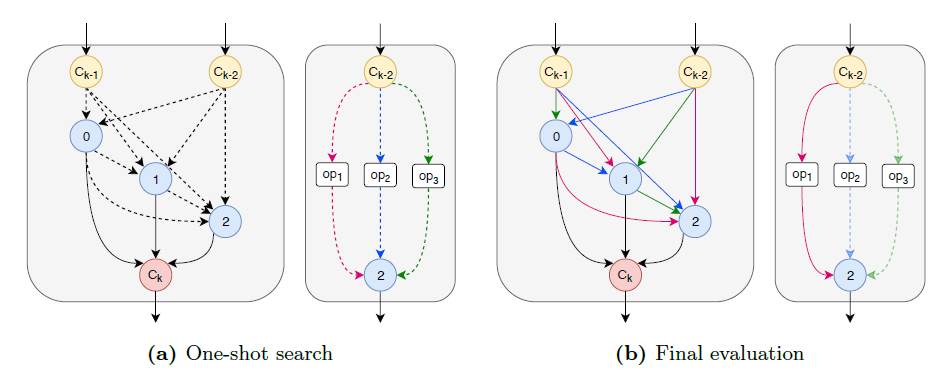
\includegraphics[scale=0.47]{images_lec7/cell_space.png}}
    	\only<1>{
	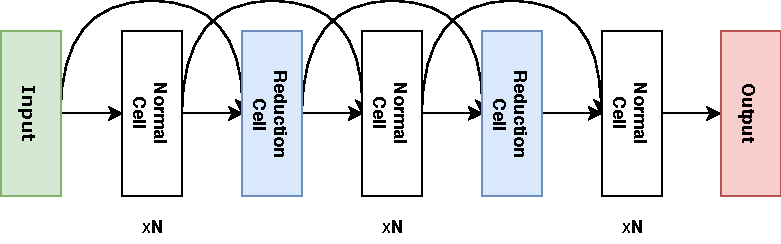
\includegraphics[scale=0.8]{images_lec7/CellBasedModel.pdf}}
	\end{centering}
	\end{figure}

\end{frame}

%----------------------------------------------------
\begin{frame}{DARTS: Continuous Relaxation}

        \begin{centering}
        {\footnotesize
        \begin{itemize}
            \item $x^{(j)} = \sum_{i<j}\tilde{o}^{(i,j)}(x^{(i)}) = \sum_{i<j}\sum_{o\in\mathcal{O}}\frac{e^{\alpha_{o}^{(i,j)}}}{\sum_{o^{\prime}\in\mathcal{O}}e^{\alpha_{o^{\prime}}^{(i,j)}}}o(x^{(i)})$
            \item $o^{(i,j)} = \argmax_{o\in\mathcal{O}}\alpha_{o}^{(i,j)}$
            \item 8 operations: $sep\_conv\_3$$\times$$3$, $sep\_conv\_5$$\times$$5$, $dil\_conv\_3$$\times$$3$, $dil\_conv\_5$$\times$$5$, $max\_pool\_3$$\times$$3$, $avg\_pool\_3$$\times$$3$, \textit{identity} and \textit{zero}
        \end{itemize}}%
        \end{centering}

        \begin{figure}[t]
        \begin{centering}
            \subfloat[][{\scriptsize Initialization}]
            {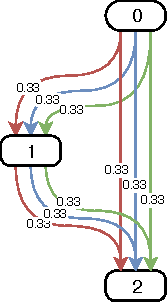
\includegraphics[scale=0.75]{images_lec7/dartsA.pdf}}
            \hspace{12mm}
            \subfloat[][{\scriptsize Search end}]
            {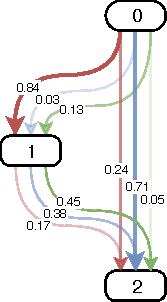
\includegraphics[scale=0.75]{images_lec7/dartsB.pdf}}
            \hspace{12mm}
            \subfloat[][{\scriptsize Final cell}]
            {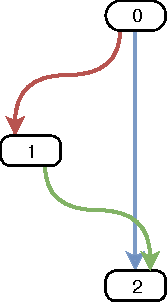
\includegraphics[scale=0.75]{images_lec7/dartsC.pdf}}
        \end{centering}
        \end{figure}

\end{frame}

%----------------------------------------------------

\begin{frame}[c]{DARTS: Architecture Optimization}

\begin{algorithm}[H]
    \footnotesize
    \caption{DARTS}
    \begin{algorithmic}
    % \ttfamily
    \INPUT{Operations $\mathcal{O}$, $\#$nodes \textit{n}, $\#$cells \textit{K}, $\#$channels \textit{C}, $\xi$,}
    \STATE \hspace{7mm} learning rates $\eta_1$, $\eta_2$
    \STATE $\texttt{model} \gets \texttt{stack}\big(DAG(\mathcal{O}, \textit{n}),K, C\big)$
    \WHILE{\textit{not converged}}
    \STATE{Update one-shot weights $\vec{w}$ by $\mathcal{L}_{train}(\vec{w}, \vec{\alpha})$}
    \STATE{Update architectural parameters $\alpha$ by $\nabla_{\alpha}\mathcal{L}_{valid}(\vec{w} - \xi \nabla_{\vec{w}}
    \mathcal{L}_{train}(\vec{w}, \alpha), \alpha)$}
    \ENDWHILE
    \OUTPUT{$\alpha$}
    \end{algorithmic}
\end{algorithm}

{\footnotesize
\begin{itemize}
    \item Optimizing both $\mathcal{L}_{train}$ and $\mathcal{L}_{valid}$ corresponds to a bilevel optimization problem:
    \begin{align}
        &\min_{\alpha} \{ f(\alpha) \triangleq \mathcal{L}_{valid}(w^*(\alpha), \alpha) \} \label{eqn:dartsbilevelA} \nonumber\\
        &s.t.\quad w^*(\alpha) = \argmin_{w} \mathcal{L}_{train}(w, \alpha)
        \nonumber
    \end{align}
    \item Approximation: $w^*(\alpha) \approx w - \xi \nabla_{w} \mathcal{L}_{train}(w, \alpha)$
    \begin{enumerate}
        \item \alert{First-order approximation:} $\xi = 0$
        \item \alert{Second-order approximation:} $\xi > 0$
    \end{enumerate}
\end{itemize}
}%

\end{frame}
%----------------------------------------------------

%----------------------------------------------------
\begin{frame}{DARTS: Deriving the final cell}
    \begin{itemize}
        \item After search finishes keep $\argmax_{o\in\mathcal{O}}\alpha_{o}^{(i,j)}$ as the optimal (non-zero) operation connecting node \textit{i} to \textit{j}
        \item Following Zoph et al, ‘17, keep top-2 incoming operations in each node
    \end{itemize}

    \begin{figure}[t]
        \begin{centering}
            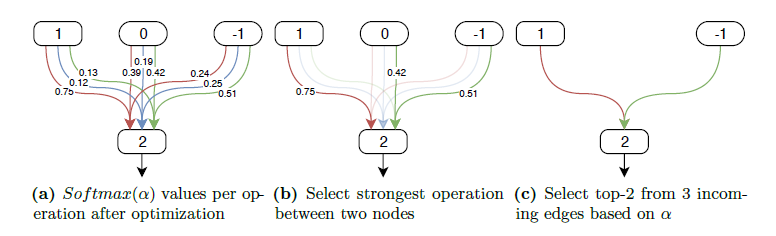
\includegraphics[scale=0.55]{images_lec7/genotype.png}
        \end{centering}
    \end{figure}

\end{frame}

%----------------------------------------------------
\begin{frame}{DARTS: Results on CIFAR-10}
\centering
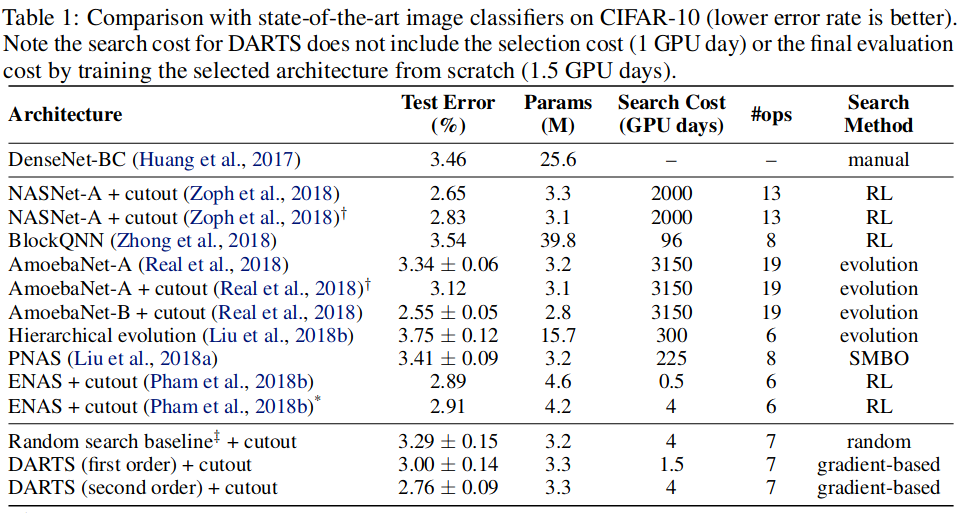
\includegraphics[width=0.85\textwidth]{images_lec7/darts_cnn_results.png}

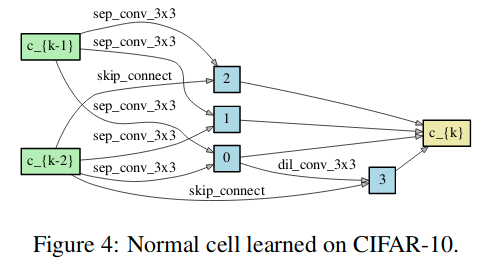
\includegraphics[width=.35\textwidth]{images_lec7/darts_normal_cell.png}
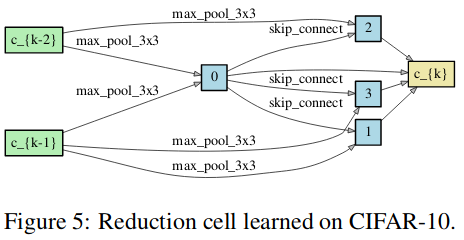
\includegraphics[width=.35\textwidth]{images_lec7/darts_reduction_cell.png}

\end{frame}

%----------------------------------------------------
\begin{frame}{Network Morphisms and Weight Inferitance}
    \begin{itemize}
    	\item \alert{Network Morphisms} \lit{Chen et al. ‘16; Wei et al. ‘16; Cai et al. ‘17}
	\begin{itemize}
		\item[--] Change the network structure, but not the modelled function
		\item[--] i.e., for every input the network yields the same output as before applying
		some network morphisms operations, such as "Net2DeeperNet", "Net2WiderNet", etc.
		\item[--] Allows efficient moves in architecture space
	\end{itemize}
    \end{itemize}

    \begin{figure}[t]
        \begin{centering}
            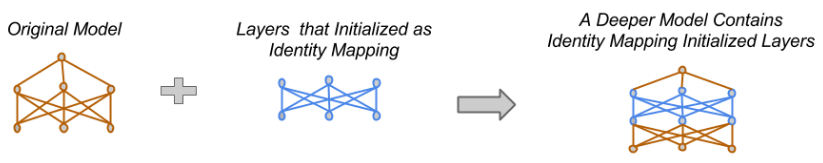
\includegraphics[scale=0.3]{images_lec7/net2deepernet.png}
        \end{centering}
    \end{figure}

\end{frame}

%----------------------------------------------------
\begin{frame}{Network Morphisms and Weight Inferitance}
    \begin{itemize}
    	\item \alert{Weight Inheritance} \lit{Real et al. ‘17; Cai et al. ‘18; Elsken et al. ‘19}
	\begin{itemize}
		\item[--] Inherit already trained weights from parent architectures to child ones
		\item[--] Do not necessary require preserving the function as in Network Morphisms
		\item[--] Network Morphisms intrinsically fulfill this property
	\end{itemize}
    \end{itemize}

    \begin{figure}[t]
        \begin{centering}
            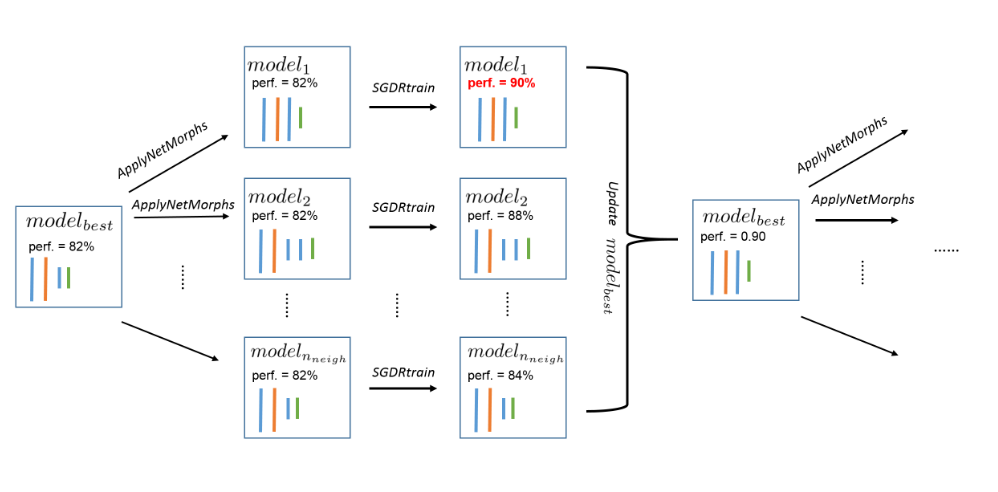
\includegraphics[scale=0.3]{images_lec7/NASH.png}
        \end{centering}
    \end{figure}

\end{frame}

%----------------------------------------------------
%----------------------------------------------------
\begin{frame}{Efficient Multi-objective NAS \litw{Elsken et al. ‘19}}
    \begin{itemize}
    	\item Trades-off network size vs. performance; maintain a \alert{Pareto front} of the \alert{2 objectives}
	\item Evolve a population of Pareto-optimal architectures over time
	\item \alert{LEMONADE}: Lamarckian Evolution for Multi-Objective Neural Architecture Design
	\begin{itemize}
		\item[--] Weight inheritance through network morphisms
		\item[--] Still cheap: 1 week on 8 GPUs
	\end{itemize}

    \end{itemize}

    \begin{figure}[t]
        \begin{centering}
            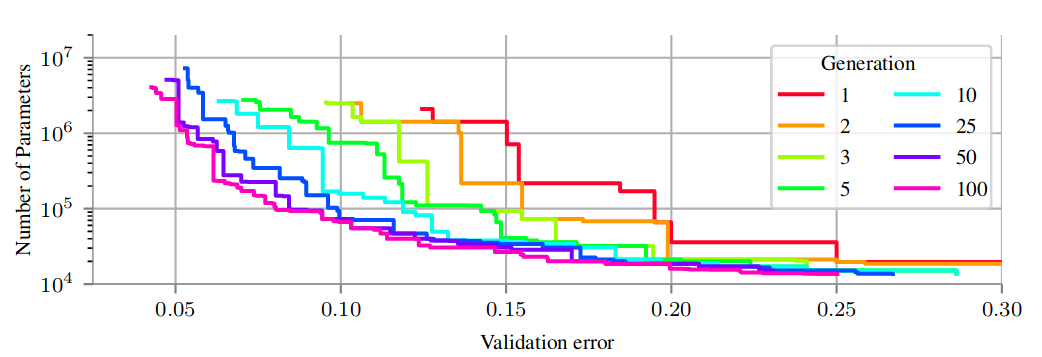
\includegraphics[scale=0.3]{images_lec7/lemonade.png}
        \end{centering}
    \end{figure}

\end{frame}
%----------------------------------------------------
%----------------------------------------------------

\begin{frame}[c]{Efficient Multi-objective NAS \litw{Elsken et al. ‘19}}
\begin{itemize}
	\item Children generation and training/evaluation of architectures 
\end{itemize}

\begin{centering}
    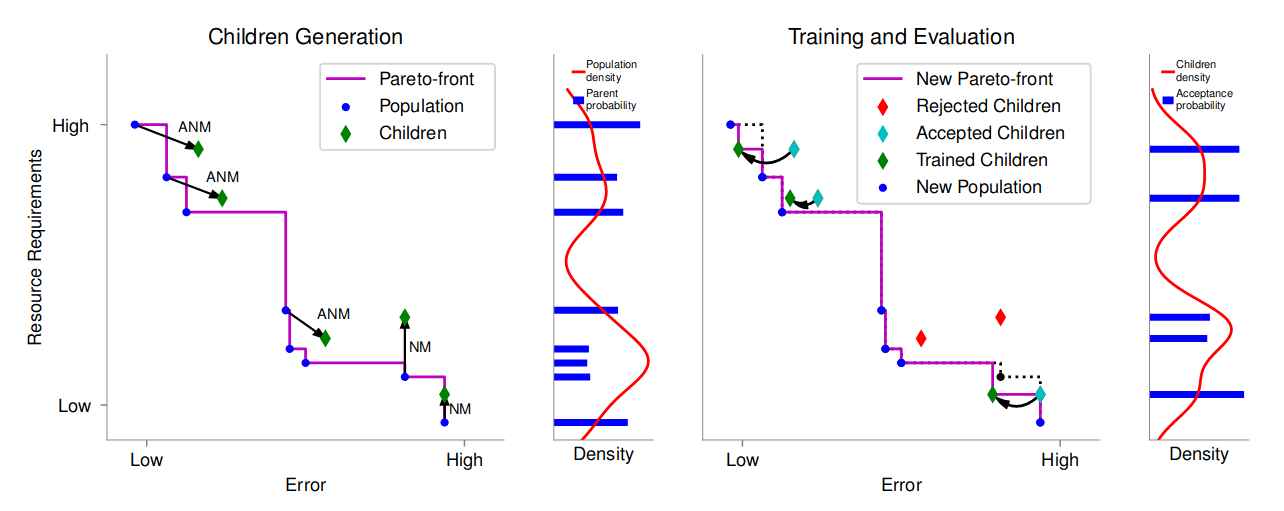
\includegraphics[scale=0.27]{images_lec7/lemonade_2.png}
\end{centering}

\end{frame}

%----------------------------------------------------
%----------------------------------------------------

\begin{frame}[t]{Are NAS strategies better than Random Search?}
\centering
\begin{itemize}
\footnotesize{
	\item \alert{Random search with weight sharing} \lit{Li and Talwalkar. ‘19}, finds model with comparable performance several SOTA NAS methods.
	\item Sciuto et al. (2019) find that a \alert{randomly sampled architecture} outperforms 3 one-shot NAS methods.
	\item Xie et al. (2019) exploit \alert{random connectivity} in a large neural networks, showing that it is comparable to other architectures found by NAS methods on ImageNet.
}
\end{itemize}

\begin{figure}[t!]
    \centering
    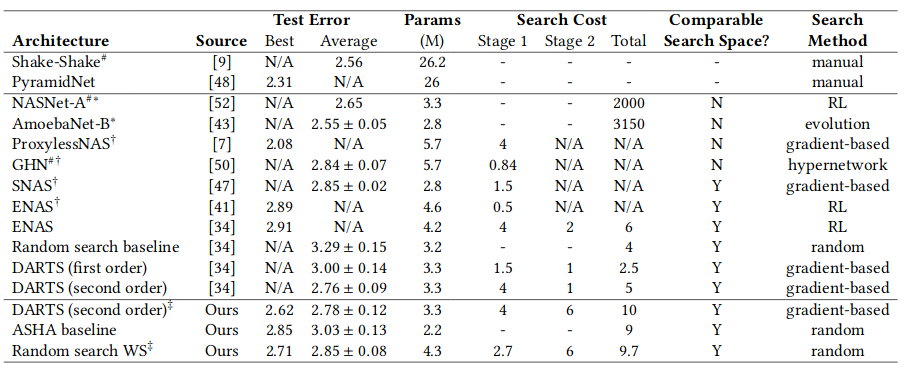
\includegraphics[width=0.59\textwidth]{images_lec7/random_cnn.png}
    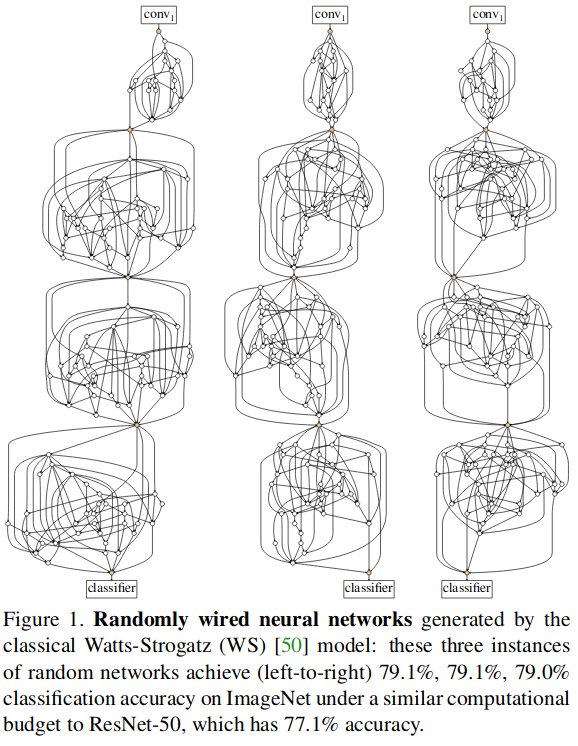
\includegraphics[width=0.3\textwidth]{images_lec7/randomly_wired.png}
\end{figure}

\end{frame}



